\chapter{Referencial Teórico}

Essa seção tem como objetivo apresentar de maneira teórica os assuntos abordados nesse projeto, conhecimento necessário pois é a base de todo o projeto que aqui será demonstrado. Temas importantes serão abordados, como funcionamento de um sistema web, metodologia de desenvolvimento de software e padrões de código. \par
Os tópicos aqui abordados servirão para nortear a metodologia proposta neste trabalho, buscando assim criar uma base sólida para os argumentos que serão apresentados. Alguns trabalhos semelhantes serão apresentados com a intenção de ajudar a contextualizar esse projeto aqui desenvolvido.


\section{Trabalho informal}\label{trabalho_informal}
Não foram encontrados artigos acerca do trabalho informal dentro das universidades, mas iremos usar como base uma pesquisa sobre o trabalho informal de jovens estudantes. Dois motivos para a inserção dos estudantes no mercado de trabalho informal é ajudar na renda familiar e obter independência financeira\cite{ferreira2009trabalhojovem}. \par
De acordo com questionário fechado e entrevistas feitas por \cite{ribeiro2005evasao}, os motivos da evasão geralmente são causados por dificuldades financeiras, vocacionais, educacionais e de dedicação. Dentre as dificuldades citadas, uma se destacou por ser o principal motivo de evasão dos estudantes entrevistado, a dificuldade financeira. Diante disso, o projeto irá atuar consistentemente em um dos motivos de evasão universitária, a dificuldade financeira, buscando assim sanar tal problema por meio de uma aplicação web.


\section{\textit{E-commerce}}\label{ecommerce}

Segundo \cite{nanehkaran2013introduction}, um \textit{e-commerce} é um mercado eletrônico de poderoso conceito e processo que revolucionou a tecnologia da informação e comunicação no campo da economia. Uma vantagem do mercado virtual é não ter necessidade de alocar um espaço físico para o mesmo, sendo possível acessa-lo a qualquer momento, de qualquer lugar do mundo. Devido aos seus vários benefícios, esse tipo de mercado se popularizou rapidamente.

A atuação do comércio eletrônico existe a cerca de 55 anos atrás, eram realizadas compras em terminais de pontos de vendas e consumidores podiam retirar dinheiro dos caixas eletrônicos\cite{wigand1997electronic}. Em 1994, quando a \textit{World Wide Web} foi introduzida de forma mais abrangente no cotidiano, tornou-se importante para a economia mundial por se tratar de um "negócio baseado na web", dessa forma esse novo mercado estava se expandindo a nível mundial\cite{nanehkaran2013introduction}.

Existem várias classificações diferentes de \textit{e-commerce}. As principais são:
\begin{itemize}  
\item B2B(\textit{Business-to-Business}): em que as transações comerciais de produtos e serviços ofertados são entre empresas;
\item B2C(\textit{Business-to-Consumer}): em que as empresasas fornecem serviços e produtos para o consumidor final;
\item C2B(\textit{Consumer-to-Business}): em que os consumidores prestam serviços para empresas;
\item C2C(\textit{Consumer-to-Consumer}): em que tais transações comerciais ocorrem entre consumidores.
\end{itemize}

\section{Aplicações web}
\label{sec:trabalhos_correlatos}

Na década de 1990 foi concebida uma nova tecnologia para a internet: a Tecnologia Web\cite{zaneti2005construcao}. O advento dessa nova tecnologia ocorreu devido a necessidade de formar um repositório de conhecimento humano \cite{lee1994www} e está baseada em troca de informações, visualização de documentos eletrônicos e mecanismos de armazenamento. \par
Essa tecnologia foi criada para divulgar o conhecimento científico, porém atualmente é utilizada como meio para vários outros segmentos de informação\cite{zaneti2005construcao}. \par
Em um modelo cliente-servidor(do inglês \textit{client-server}), o navegador faz o papel do cliente, responsável assim por fazer requisições ao servidor. Por sua vez, o servidor é responsável por receber e tratar a requisição feita pelo cliente, logo após ele irá devolver uma resposta para o mesmo\cite{sousa2016desenvolvimento}. A Figura \ref{fig:web} exemplifica muito bem essa comunicação.

Uma aplicação web é um sistema projetado para ser executado em um navegador, essa é sua principal vantagem, visto que não será necessário alguns pré-requisitos como o uso de um sistema operacional em específico, por exemplo. Essa característica multiplataforma é ótima em relação a mobilidade e flexibilidade, pois em qualquer lugar/dispositivo que contém um navegador será possível acessar a aplicação. Além disso, as tecnologias para desenvolvimento web evoluíram muito, atualmente é possível fazer layouts que se adéquam aos \textit{smartphones}, buscando assim uma melhor experiência para o usuário\cite{pandey2013responsive}. \par
O sistema aqui proposto se encaixa muito bem em um modelo web, devido aos seus atores da aplicação necessitarem de portabilidade da aplicação, pois os mesmo se encontram em uma rotina corriqueira, devido ao deslocamento entre sua casa, estágio, universidade e afazeres em geral. Para que seja possível criar uma plataforma web, será necessário escolhe uma linguagem de programação entre as diversas disponíveis para isso.

\begin{figure}[htbp!]
  \centering
  \caption{Modelo cliente-servidor}
  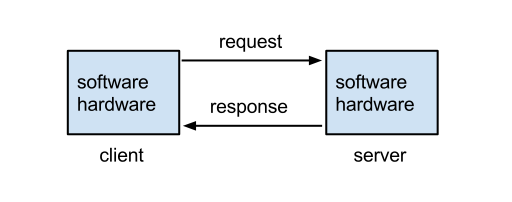
\includegraphics[width=1\textwidth]{figs/web.png}
    \legend{Fonte: https://commons.wikimedia.org/wiki/File:Client-server\_model.svg acessado dia 15 de dezembro de 2019 às 23:26}
    \label{fig:web}
\end{figure}

\section{Linguagem Ruby}
Desenvolvida em 1995 por Yukihiro Matsumoto, Ruby é uma linguagem interpretada que inicialmente tinha objetivos muito semelhantes a linguagem Python\cite{purer2009phpvspythonvsruby}. Dinâmico e de código fonte aberto, a linguagem tem foco na simplicidade e produtividade, possui uma sintaxe elegante, natural e fácil de ler e escrever \cite{siteruby}. \par
Ruby segue o princípio de pouca surpresa, isso significa que a linguagem foi construída para ser intuitiva e com comportamentos esperados para o programador\cite{purer2009phpvspythonvsruby}. Diante disso, a curva de aprendizado da linguagem se torna muito baixa, encorajando assim outras pessoas a contribuir com o projeto desenvolvido aqui. A linguagem Ruby dispõe de alguns \textit{frameworks} para facilitar seu desenvolvimento.

%\subsection{RGB}
%Amplamente conhecido, é um modelo de cor aditiva onde as cores vermelho, verde e azul são combinadas em diferentes intensidades produzindo outras cores. O RGB (vermelho, verde e azul) são chamadas de cores primárias.

%Na Figura \ref{fig:cor_RGB} podemos ver a representação do espaço de cor RGB.

%\begin{figure}[hbtp!]
% \centering
% \caption{Representação do espaço de cor RGB}
% \includegraphics[scale=0.07]{figs/RGB.png}
% \legend{Fonte: \cite{cor_RGB}}
% \label{fig:cor_RGB}
%\end{figure}

%\subsection{HSV}
%Hue (matiz): define o componente de cor, ou a posição no círculo.

%Saturation (saturação): define o quão "pura" é a cor, ou se ela está
%misturada com outras cores (complementar), tornando-a mais pálida.

%Value (valor/brilho): define a quantidade de luz na mistura, quanto
%mais luz mais clara a cor (na ausência de valor, a imagem é toda
%preta).

%Na Figura \ref{fig:cor_HSV} podemos ver a representação do espaço de cor HSV.

%\begin{figure}[hbtp!]
% \centering
% \caption{Representação do espaço de cor HSV}
% \includegraphics[scale=0.07]{figs/HSV.png}
% \legend{Fonte: \cite{cor_HSV}}
% \label{fig:cor_HSV}
%\end{figure}

\section{\textit{Framework}}
Em desenvolvimento de software, \textit{framework} é uma concepção de vários códigos comuns entre diversos projetos, buscando assim um kit de ferramentas genéricos para ser usado de acordo com a necessidade de cada projeto a ser implementado em cima dele. Segundo Fayad e Schmidt, framework é um conjunto de classes que colaboram para realizar uma responsabilidade para um domínio de um subsistema da aplicação\cite{frameworkwikipedia}. \par
As principais vantagens de \textit{frameworks} são: maior facilidade para debugar algum erro de implementação, foco na abstração de soluções do problema proposto, eficiência na resolução dos problemas e melhora no uso dos recursos\cite{frameworkwikipedia}. \par
O Ruby on Rails(RoR) teve sua primeira versão lançada em dezembro de 2005, foi desenvolvido pela 337Signal Inc com o objetivo de criar o projeto Basecamp, um gerenciamento colaborativo de projetos. Escrito em linguagem Ruby, RoR é um \textit{framework full-stack}(ou seja, possui ferramentas para desenvolvimento \textit{frontend} e \textit{backend}) para desenvolvimento de aplicativos web baseados em banco de dados\cite{plekhanova2009evaluating}. \par
Esse \textit{framework} foi escolhido para o projeto por alguns motivos, tanto pessoais como técnicos. Foi levado em consideração uma forte familiaridade da equipe executante do atual projeto com a linguagem de programação Ruby, devido aos mesmos utilizarem ela na vida acadêmica e profissional. Diante disso, a execução do projeto seria mais ágil e eficaz. Quando comparado com outros \textit{frameworks}, como Laravel, RoR é um dos mais utilizados, tem atualizações frequentes e uma vasta comunidade de código aberto, nitidamente terá um futuro seguro no mundo na programação \cite{verma2014mvc}.

Bootstrap é um \textit{framework web frontend} popular framework de código fonte aberto que oferece assistência a fácil e rápido desenvolvimento de aplicações web, baseando-se em modelo de design, teoria das cores e tipografia esse \textit{framework} serve para criar uma identidade visual forte e amigável para sistemas web, buscando melhorar o contato do usuário com o sistema\cite{shah2015responsive}. Esse \textit{framework} conta atualmente com uma enorme popularidade que vem crescendo todos os dias \cite{jain2014review}. \par

%Na próxima seção é apresentado o OpenCV e alguns algoritmos que auxiliaram no processo de segmentação e que foram analisados neste trabalho.

%\newpage
%\subsection{Baseado em detecção de bordas}
%Primeiro aplica-se o método da morfologia matemática para detecção de bordas, que podem ser o de Sobel, Canny, Laplaciana, Prewit ou Roberts. Em seguida é feita um agrupamento de pixels detectados como bordas, a partir de um algoritmo de união ou realce de bordas, que permite determinar de maneira mais precisa o contorno dos objetos de uma imagem.
%Na Figura \ref{Border Detection} pode ser visto a utilização da técnica de detecção de bordas em manchas na pele.

%\begin{figure}[hbpt!]
% \centering
% \caption{Exemplo de segmentação utilizando detecção de bordas}
% \includegraphics[scale=0.3,angle=90]{figs/algoritmos/anisotropic_dermoscopy.png}
% \legend{Fonte: \cite{anisotropic_dermoscopy}}
% \label{Border Detection}
%\end{figure}

%\subsection{Baseado em regiões}
%Um conjunto de pixels que possuem determinado grau de similaridade, são tidos como regiões. No método de segmentação baseado em regiões, cada região é composta por pixels com um valor similar, baseado em um critério de similaridade. Na Figura \ref{Baseado em regiões} pode-se ver a técnica sendo aplicada na segmentação do milho e ervilha, ou de feijões de cores e tamanhos diferentes.

%\begin{figure}[hbpt!]
%\centering
%\caption{Exemplo de segmentação baseado em regiões}
%\begin{minipage}{.5\textwidth}
  %\centering
  %\includegraphics[width=.75\linewidth]{figs/opencv/region_growing_1.png}
%   \label{fig:test1}
%\end{minipage}%
%\begin{minipage}{.5\textwidth}
  %\centering
  %\includegraphics[width=.75\linewidth]{figs/opencv/region_growing_2.pn%g}
%   \label{fig:test2}
%\end{minipage}
%\legend{Fonte: \cite{region_growing}}
%\label{Baseado em regiões}
%\end{figure}


%\subsection{Transformação divisória (Watershed)}

%São algoritmos que possuem como base a morfologia matemática, que permite extrair as bordas existentes em uma imagem, e é também uma técnica de segmentação baseada em regiões. Imagina-se os valores dos pixels da imagem como um gráfico topográfico 3D, onde o 'x' e 'y' são coordenadas do plano e 'z' são os valores dos pixels. O objetivo principal é encontrar as linhas divisórias em uma imagem para separar diferentes regiões, que correspondem aos mínimos do gradiente morfológico. Na Figura \ref{Watershed} pode ser visto a utilização da técnica do watershed para segmentação de uma imagem.

%\begin{figure}[hbpt!]
% \centering
% \caption{Exemplo de segmentação utilizando watershed}
% \includegraphics[scale=0.4]{figs/algoritmos/elephant.jpg}
% \legend{Fonte: \cite{watershed_citation}}
% \label{Watershed}
%\end{figure}

\section{Banco de dados}
\label{sec:opencv}

Segundo \cite{ceri2013logic}, “sistemas de banco de dados lidam com grandes coleções de dados compartilhados e com memória de massa e fornecem a tecnologia para suportar recuperação eficiente e atualização confiável de dados persistentes”. \par
O banco de dados baseado no modelo relacional foi arquitetado há mais de 35 anos com o objetivo de atender ao processamento de dados, desde então, tornou-se a melhor opção para armazenar informações. O modelo Não Relacional(NoSQL) é baseado em arquivos e foi desenvolvido por Carlo Strozzi em 1998, modelo ao qual omite o uso da linguagem SQL.\cite{mohamed2014relationalvsnosql} \par
No projeto em questão será utilizado o modelo relacional, pois o NoSQL ainda não atingiu uma maturidade completa devido ao seu surgimento recente, outro ponto é a escassez em segurança dos bancos NoSQL como demonstrado na tabela 1\cite{mohamed2014relationalvsnosql}: \par

\begin{table}[ht]
\centering
\caption{Tabela de comparação entre banco de dados relacionais e não relacionais}
\label{tab:sqlvsnosql}
% \begin{flushright}
% \footnotesize
% (continua)
% \end{flushright}
\resizebox{\textwidth}{!}{%
\begin{tabularx}{1\textwidth} { 
  | >{\raggedright\arraybackslash}X 
  | >{\raggedright\arraybackslash}X 
  | >{\raggedright\arraybackslash}X | }
 \hline
 Categoria & Modelo relacional & Modelo não-relacional \\
 \hline
 Autenticação  & Todos os bancos de dados relacionais vieram com mecanismo de autenticação e podem escolher qualquer um desses mecanismos a serem usados.  & Muitos bancos de dados NoSQL, por padrão, não vêm com mecanismo de autenticação ou autorização, mas podem usar algum método externo para executar esta operação.  \\
\hline
Integridade dos dados & As propriedades ACID(acrônimo de Atomicidade, Consistência, Isolamento e Durabilidade) usadas nos bancos de dados relacionais garantem que as transações do banco de dados sejam processadas com confiabilidade, garantindo a integração dos dados. & Eventualmente consistente é um dos princípios das propriedades BASE, portanto, a integridade dos dados nem sempre é alcançada nos bancos de dados NoSQL. \\
\hline
Confidencialidade & A confidencialidade dos dados geralmente é alcançada no banco de dados relacional porque foi usada técnicas de criptografia para armazenar dados criptografados. & A confidencialidade dos dados não é alcançada, porque geralmente os dados são armazenados de forma clara. \\
% \hline
% Auditoria & Fornecer mecanismos auditar que permita escrever para o arquivos syslog ou xml do banco de dados, e alguns dar uma auditoria mais avançada. & A maioria do NoSQL bancos de dados não fornecer auditoria. Existem alguns bancos de dados que fornecem auditoria como Couchdb que guarda o nome de usuário e senha no log arquivo que é claro compromete a segurança. \\
\hline
Comunicação com o cliente & Os bancos de dados relacionais oferecem mecanismo seguro de comunicação com o cliente usando protocolos de criptografia e \textit{Secure Sockets Layer}(SSL). & A maioria dos bancos de dados NoSQL não oferecem mecanismos de comunicação segura com o cliente. \\
\hline
\end{tabularx}%
}
\end{table}

% \begin{table}[ht]
% \centering
% Tabela \ref{tab:sqlvsnosql} – Tabela de comparação entre banco de dados relacionais e não relacionais
% \begin{flushright}
% \footnotesize
% (conclusão)
% \end{flushright}
% \resizebox{\textwidth}{!}{%
% \begin{tabularx}{1\textwidth} { 
%   | >{\raggedright\arraybackslash}X 
%   | >{\raggedright\arraybackslash}X 
%   | >{\raggedright\arraybackslash}X | }
%  \hline
%  Categoria & Modelo relacional & Modelo não-relacional \\
% \hline
% Comunicação com o cliente & Os bancos de dados relacionais oferecem mecanismo seguro de comunicação com o cliente usando protocolos de criptografia e \textit{Secure Sockets Layer}(SSL). & A maioria dos bancos de dados NoSQL não oferecem mecanismos de comunicação segura com o cliente. \\
% \hline
% \end{tabularx}%
% }
% \end{table}
% \pagebreak

\section{Engenharia de software}

Segundo \cite{van2008software}, engenharia de software é o estabelecimento e uso dos princípios da engenharia para construir um software que funcione em máquinas reais e seja confiável. Por um lado engenharia de software possui características explícitas de produção e engenharia devido ao processo de criação do produto(software). Por outro lado é exigido uma melhoria contínua e sequencial da qualidade do produto e do processo de criação do software, nesse contexto é enxergado como ciência\cite{travassos2002introducao}.

%O OpenCV conta com mais de 150 métodos de conversão do espaço de cores, mas o BGR <-> Cinza e BGR <-> HSV são os mais utilizados. A função tem o escopo Imgproc.cvtColor(imagem\_entrada, imagem\_saida, flag) onde \textit{flag} determina o tipo de conversão.

%Para RGB -> Cinza utiliza-se a \textit{flag} Imgproc.COLOR\_BGR2GRAY e para RGB -> HSV utiliza-se a \textit{flag} cv2.COLOR\_BGR2HSV. Um exemplo de conversão de escala de cor de RGB (Figura \ref{fig:lenna_rgb}) para Cinza (Figura \ref{fig:lenna_gray}) pode ser visualizado na Figura \ref{fig:rgb2gray}.

\subsection{Padrão de Projeto MVC (Model View Controller)}
\label{subsec:thresholding}

O padrão \textit{model-view-controller}(MVC) é um padrão de projeto(do inglês \textit{design pattern}) de apresentação/abstração/controle utilizado para arquitetar sistemas de softwares \cite{leff2001webmvc}. O paradigma MVC separa a aplicação em três tipos de objetos, cada um especializado em sua tarefa, são elas: Modelo(\textit{Model}), Visão(\textit{View}) e Controlador(\textit{Controller}). \par
O \textit{Model} gerencia e valida o comportamento dos dados da aplicação, conversando com o banco de dados, por exemplo. A \textit{View} é a parte gráfica da aplicação ao qual irá interagir visualmente com o usuário. O \textit{Controller} interpreta, ordena e responde a requisições feitas pelos usuários\cite{burbeck1997applications}. A Figura \ref{fig:mvc} exemplifica muito bem a abordagem do MVC. \par

\begin{figure}[htbp!]
  \centering
  \caption{Fluxo do padrão MVC}
  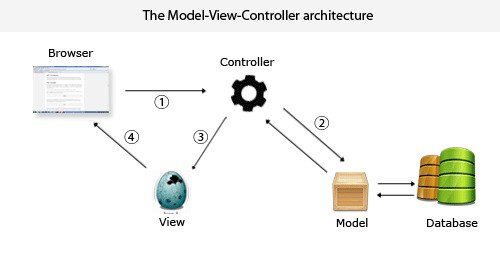
\includegraphics[width=1\textwidth]{figs/mvc.jpg}
    \legend{Fonte: https://www.cuelogic.com/blog/hello-world-in-ruby-on-rails-and-folder-structure acessado dia 16 de dezembro de 2019 às 08:15}
    \label{fig:mvc}
\end{figure}

%As transformações morfológicas são operações simples baseadas na forma da imagem. Normalmente utilizado em imagens binárias. A função necessita de dois parâmetros, um é a imagem de entrada, o outro é o elemento estruturante, ou kernel, que decide a natureza da operação. Duas operações morfológicas básicas são a erosão e a dilatação.

%A ideia básica da erosão é servir como uma erosão do solo, removendo ruídos ou reduzindo bordas do objeto. A dilatação é a ideia oposta da erosão, cujo objetivo é aumentar as bordas do objeto. Normalmente, em caso de remoção de ruídos, a erosão é sucedida de dilatação.

\subsection{Testes automatizados}

Segundo \cite{mathur1991performance}, “A confiabilidade do software é uma medida do desempenho de um programa em seu ambiente operacional”. Para elevar a confiabilidade é necessário recorrer a métodos de testes. Existem vários tipos de testes de softwares, e cada um se aplica em um estágio do desenvolvimento do software, pois cada um tem objetivos diferentes\cite{nidhra2012black}. \par
No projeto proposto será implementado tais testes: \par
\begin{itemize}
\item Testes unitários, aos quais testa um componente isolado ou classe do sistema;
\item Testes de integração, aos quais combinam vários componentes do software para testar se funcionam de maneira satisfatória;
\item Teste de segurança, responsável por testar se os dados são acessados de maneira segura.
% \item Teste funcional, encarregado de testar se os requisitos funcionais foram alcançados.
\end{itemize}
Testes funcionais, de sistema, de aceitação e beta não foram incluídos devido a sua característica de necessitar pessoas independentes ao projeto para testar o software.


\section{Projetos de código fonte aberto}

OSS(\textit{Open Source Software}) é um termo usado para designar um software desenvolvido e lançado sob algum tipo de licença de código aberto. Atualmente existem várias licenças com uma gama de características diferentes, mas todas necessitam da permissão do código fonte do software\cite{crowston2003defining}.

Algumas vantagens de projetar um OSS são:
\begin{itemize}  
\item Oferta gratuita de código aumentará a participação de mercado\cite{fitzgerald2006transformation};
\item Construir uma base de desenvolvimento em torno da ferramenta aumentar a sustentabilidade a longo prazo\cite{nyman2011forking};
\item O conjunto crescente de partes interessadas resulta em melhorias adicionais sucessivas no software\cite{heron2013open};
\item Replicação dos resultados obtidos neste projeto.
\end{itemize}


\section{Trabalhos correlatos}
\label{sec:java}

Foram pesquisados alguns trabalhos, porém nenhum se encaixou perfeitamente com os objetivos do projeto, ao qual tem como premissa estar inserido no ambiente acadêmico. Entretanto, alguns projetos têm cunho semelhante, como o Mercado Livre e OLX. \par

\subsection{Mercado Livre}

O Mercado Livre é uma empresa de tecnologia que tem como objetivo democratizar o comércio eletrônico oferecendo uma ótima plataforma e serviços que seja possível comprar, pagar, vender e anunciar seus negócios na internet \cite{brasil_2019}.

Como pode ser observado na Figura \ref{fig:livre_5}, o Mercado Livre é o 5º site mais acessado do Brasil em 2017, o Mercado Livre conta com mais de 211 milhões de usuários registrados na América Latina, 52 milhões de visitantes únicos por mês e é o maior site de \textit{e-commerce} do Brasil.

\begin{figure}[htbp!]
  \centering
  \caption{Mercado Livre é o 5º site mais acessado do Brasil}
  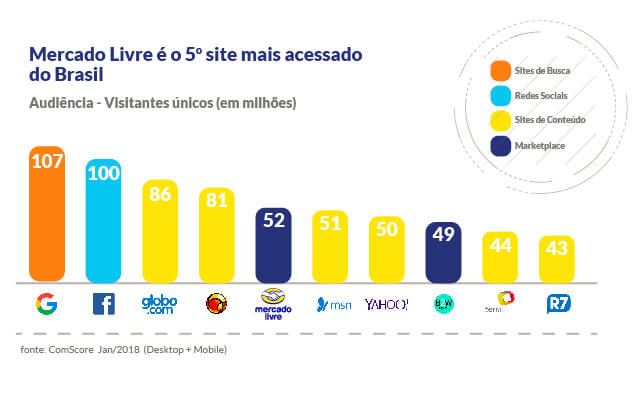
\includegraphics[width=0.9\textwidth]{figs/ml1.jpg}
    \legend{Fonte: https://ideias.mercadolivre.com.br/sobre-mercado-livre/tudo-o-que-voce-precisa-saber-sobre-o-mercado-livre/ acessado dia 4 de fevereiro de 2020 às 17:38}
    \label{fig:livre_5}
\end{figure}

O Mercado Livre oferece um conjunto de soluções para melhorar e potencializar a eficácia de comprar e vender pela internet, fomentar o desenvolvimento de uma comunidade empreendedora e diversificar os produtos disponíveis no mercado. A Figura \ref{fig:livre} apresenta o Modelo Canvas do Mercado Livre.

\subsection{OLX}

OLX é uma empresa global de \textit{e-commerce} do tipo C2C, sediada em Amsterdam, Países Baixos. Fundada em 2006, a empresa chegou ao Brasil apenas em 2010 por meio de parcerias com dois grupos de mídias e investimentos em marketplaces, Naspers e Schibsted.

O modelo de negócio da OLX tem como objetivo articular e facilitar a venda de produtos novos e usados entre vendedores e compradores. OLX tem como público alvo as pessoas físicas, permitindo que elas anunciem facilmente seus produtos com fotos, descrição, preço e oferece uma comunicação direta entre o comprador e o vendedor por meio de um chat na própria plataforma.

A grande vantagem da OLX é não realizar cobrança de taxas pelos anúncios no sistema, isso faz com que os preços dos itens sejam mais em conta. A plataforma oferece vários filtros para pesquisa dos produtos anunciados, tais filtro são associados a categoria do produto, como também em relação ao local em que se encontra esse produto dividindo em estados, cidades, ou zonas de DDD. A Figura \ref{fig:olx} apresenta o Modelo Canvas do OLX.

\begin{figure}[h]
  \centering
  \caption{Modelo Canvas do Mercado Livre}
  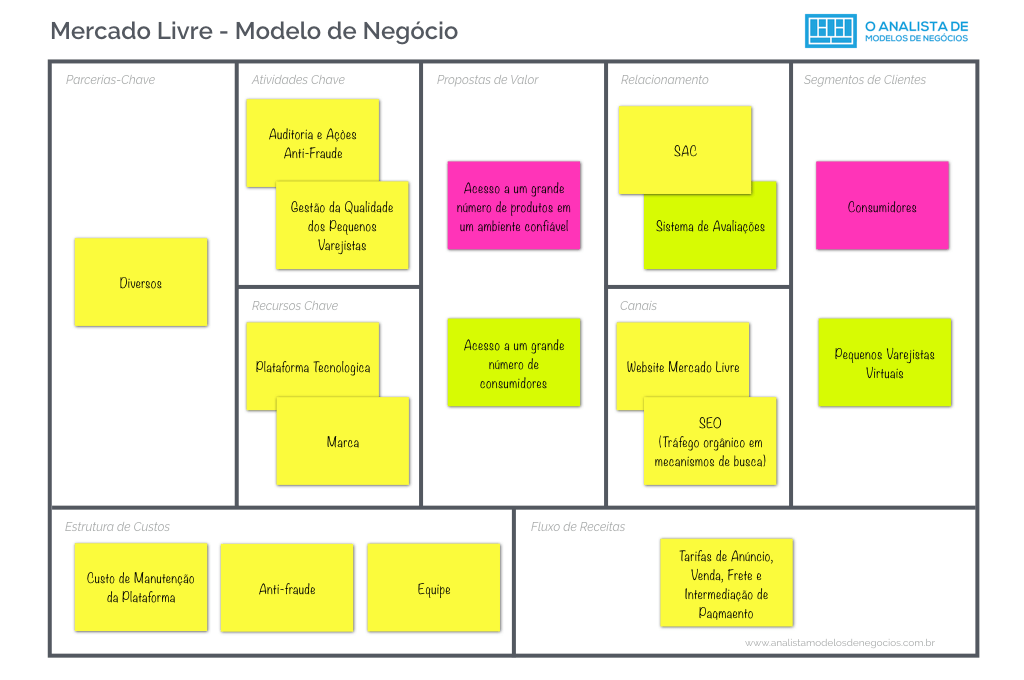
\includegraphics[width=1\textwidth]{figs/canvas_livre_1.png}
    \legend{Fonte: https://analistamodelosdenegocios.com.br/modelo-de-negocio-mercado-livre/ acessado dia 5 de fevereiro de 2020 às 11:04}
    \label{fig:livre}
\end{figure}

\clearpage
\begin{figure}[ht]
  \centering
  \caption{Modelo Canvas do OLX}
  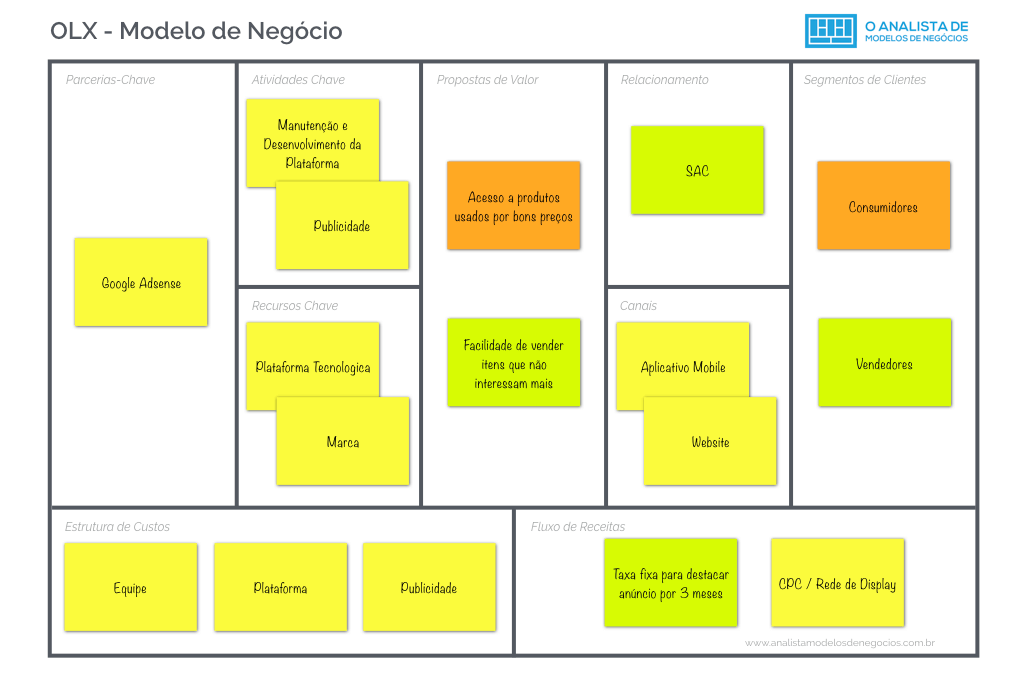
\includegraphics[width=1\textwidth]{figs/canvas_olx_1.png}
    \legend{Fonte: https://analistamodelosdenegocios.com.br/modelo-de-negocio-olx/ acessado dia 5 de fevereiro de 2020 às 11:10}
    \label{fig:olx}
\end{figure}